\section{Resultados}

\subsection{Complejidad algorítmica}

El algoritmo \ref{alg:FAP} presenta una complejidad cuadrática, esto es debido a que en el ciclo de la linea 9, este recorre todas las conexiones posibles de todos los nodos, que contemplando el caso en que todos los nodos esten conectados entre si, este tendra una cantidad de n(n-1). Lo que se ve reducido a tener $n^2$.

\subsection{Costos obtenidos}

Las medidas de tendencia central y percentiles obtenidos de los resultados del algoritmo \ref{alg:FAP} con 34, 39 y 49 canales disponibles se encuentran en la tabla \ref{table:central_tendency}.

\begin{table}[H]
    \centering
    \begin{tabular}{ccccccc} \hline
        \multicolumn{1}{c}{\begin{tabular}[c]{@{}c@{}}\textbf{Canales}\\ \textbf{disponibles}\end{tabular}} & \textbf{Media} & \textbf{Mínimo} & \textbf{25 \% } & \textbf{50\%} & \textbf{75\%} & \textbf{Máximo} \\ \hline
        \textbf{34}                                   & 8.55$x10^9$    & 7.70$x10^9$     & 8.40$x10^9$     & 8.60$x10^9$   & 8.70$x10^9$   & 8.903$x10^9$    \\
        \textbf{39}                                   & 7.24$x10^9$    & 6.70$x10^9$     & 7.10$x10^9$     & 7.25$x10^9$   & 7.40$x10^9$   & 7.608$x10^9$    \\
        \textbf{49}                                   & 5.39$x10^9$    & 4.90$x10^9$     & 5.30$x10^9$     & 5.40$x10^9$   & 5.50$x10^9$   & 5.709$x10^9$    \\ \hline
    \end{tabular}
    \caption{Medidas de tendencia central y percentiles de los costos mínimos obtenidos con el algoritmo \ref{alg:FAP} para 34, 39 y 49 canales disponibles.}
    \label{table:central_tendency}
\end{table}


En la figura \ref{fig:boxplot} se muestra graficamente la distribución de los costos mínimos obtenidos a partir del algoritmo \ref{alg:FAP}. Se observa que a mayor disponibilidad de canales se tienen disponibles, el costo disminuye. La variabilidad de los resultados con relación a su media es semejante en los tres casos.

\begin{figure}[H]
    \centering
    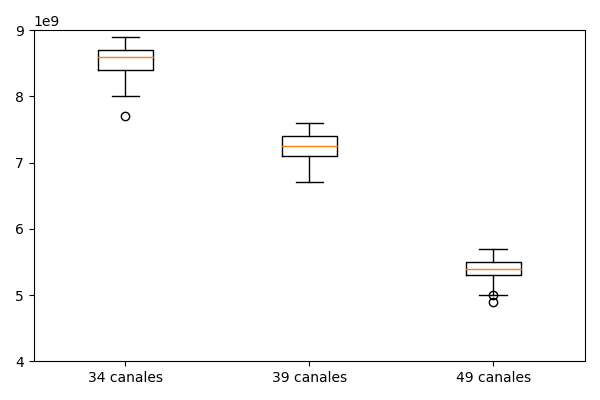
\includegraphics[width=10cm]{Graphics/boxplot.png}
    \caption{Boxplot de los costos mínimos obtenidos con el algoritmo \ref{alg:FAP} para 34, 39 y 49 canales disponibles.}
    \label{fig:boxplot}
\end{figure}

